\subsection{Calculation results}

We select several particles ($100$th, $200$th, $\ldots$, $1000$th) and plot their traces
from $t = 390$ to $t = 500$ (i.e., at $T \approx 1.073$) in Figure~\ref{fig:traces}.
The figure shows that these particles are wandering around a certain
range. The straight lines passing through the box does not mean they just at a very
large speed, since after thermalization, the speed of particles would not change so
much. These lines just indicate that these particles move out the current cell,
and their images reappear from the other side of the cell, as required by the PBCs.

\begin{figure}
    \centering
    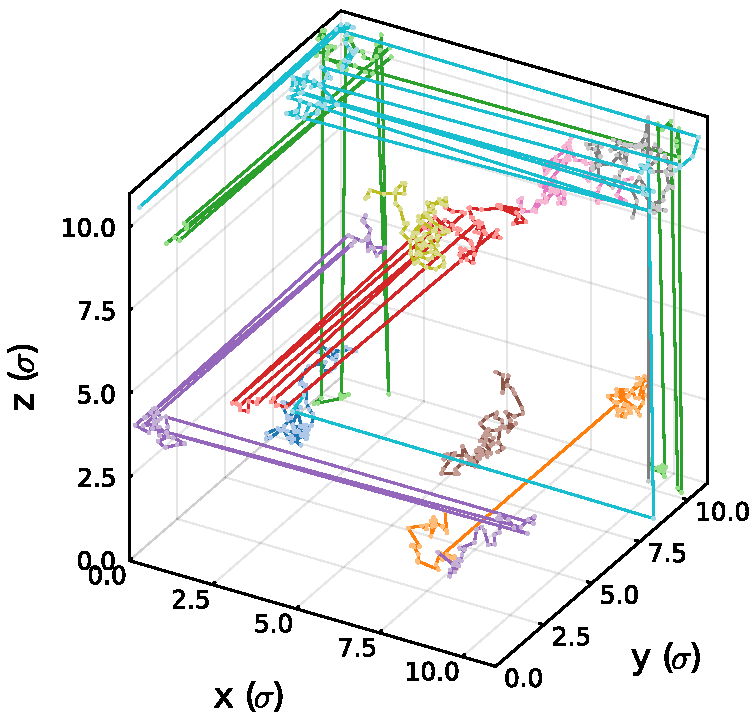
\includegraphics[width=0.8\textwidth]{traces}
    \caption{The traces of the $100$th to $1000$th particles from $t = 390$ to $t = 500$.}
    \label{fig:traces}
\end{figure}

Now let us calculate the \ce{Ar} system's thermodynamic properties.

The pressure is calculated from the virial theorem, as shown in \eqref{eq:P}
%
\begin{equation}\label{eq:P}
    P = \rho k_B T - \frac{ \rho }{ 3N } \sum_{i=1}^{N} \sum_{\alpha=1}^{3}
    \biggl \langle r_i^\alpha \frac{ \partial u }{ \partial r_i^\alpha } \biggr \rangle,
\end{equation}
%
where $i$ labels all the particles, and $\alpha$ labels the three spatial dimensions.
Its dimensionless form is shown in \eqref{eq:Pdimensionless}\cite{thijssen_2007}:
%
\begin{equation}\label{eq:Pdimensionless}
    P = 1 + \frac{ 1 }{ 3N } \sum_{i=1}^{N}
    \langle \bm{r}_i \cdot \bm{F}_i \rangle,
\end{equation}
%
where $\bm{F}_i$ is the total force on the $i$th particle, and $\bm{r}_i$ is the
position of the particle.
